\documentclass[11pt]{beamer}
\usepackage{helvet} %font
\beamertemplatenavigationsymbolsempty
\usetheme{JuanLesPins}
\usefonttheme{structurebold}

\usepackage[french]{babel}
\usepackage[utf8]{inputenc}
\usepackage[T1]{fontenc}
\usepackage{amssymb,amsmath}
\usepackage{tikz}
\usepackage{xcolor,colortbl}
\usetikzlibrary{arrows,positioning}
\usepackage{listings}
\usepackage{wasysym}

\newenvironment{slide}[1]{%
\begin{frame}[environment=slide]
\frametitle{#1~\hfill~
\includegraphics[height=1.2cm]{./epitech.png}}
}{%
\end{frame}
}
\setbeamercolor{structure}{fg=red}
\setbeamercolor{frametitle}{bg=black,fg=white}
\definecolor{gris}{gray}{0.6}
\definecolor{grisclair}{gray}{0.9}
\definecolor{gray0.9}{gray}{.95}
\definecolor{gray0.8}{gray}{.85}
\definecolor{gray0.7}{gray}{.75}
\definecolor{gray0.6}{gray}{.7}
\definecolor{gray0.55}{gray}{.65}
\definecolor{gray0.5}{gray}{.6}
\definecolor{gray0.45}{gray}{.575}
\definecolor{gray0.4}{gray}{.55}
\definecolor{gray0.35}{gray}{.525}
\definecolor{gray0.3}{gray}{.5}

\title{Du Data brut au Matching optimal}
\author{}
\date{}

%\AtBeginSection[] {
%  \begin{frame}<beamer>{}
%    \tableofcontents[currentsection]
%  \end{frame}
%}

	
\newcommand{\Python}[1]{
	{\small	\lstinputlisting[language=Python]{./#1.py}}
}

\newcommand{\elimine}[1]{{\textcolor{lightgray}{#1}}}


\begin{document}

\section{Introduction}

\part{Maximiser le nombre d'allocations}

\section{Maximiser le nombre d'allocations}

\subsection{Présentation du problème de MATCHING}

\begin{slide}{Ressources nécessaires}

\begin{itemize}
	\item Python 3.x (depuis le site officiel)
	\item un éditeur (notepad++,scribes,gedit,sublimetext)
	\item IDE (thonny,pycharm,pyzo)
	\item les données : \texttt{ouralou.fr/Resources/epitech.zip}
	\item papier + crayon
	\item présentation de graphes (graphviz)
\end{itemize}

\end{slide}

\begin{slide}{Un graphe de compatibilité}

\begin{tikzpicture}

\node (1) at (0,0){Ainur};
\node (2) at (0,1){Béatrice};
\node (3) at (0,2){Claude};
\node (4) at (0,3){Denis};
\node (5) at (4,0){Eléonore};
\node (6) at (4,1){François};
\node (7) at (4,2){Genki};
\node (8) at (4,3){Hussein};
\draw (1) -- (5);
\draw (1) -- (7);
\draw (2) -- (5);
\draw (2) -- (6);
\draw (2) -- (8);
\draw (3) -- (6);
\draw (4) -- (6);
\draw (4) -- (8);

\end{tikzpicture}

\end{slide}

\begin{slide}{Une allocation sous-optimale}

\begin{tikzpicture}

\node (1) at (0,0){Ainur};
\node (2) at (0,1){Béatrice};
\node (3) at (0,2){Claude};
\node (4) at (0,3){Denis};
\node (5) at (4,0){Eléonore};
\node (6) at (4,1){François};
\node (7) at (4,2){Genki};
\node (8) at (4,3){Hussein};
\draw[ultra thick,red] (1) -- (5);
\draw (1) -- (7);
\draw (2) -- (5);
\draw[ultra thick,red] (2) -- (6);
\draw (2) -- (8);
\draw (3) -- (6);
\draw (4) -- (6);
\draw[ultra thick,red] (4) -- (8);

\end{tikzpicture}

\end{slide}

\begin{slide}{Une allocation optimale}

\begin{tikzpicture}

\node (1) at (0,0){Ainur};
\node (2) at (0,1){Béatrice};
\node (3) at (0,2){Claude};
\node (4) at (0,3){Denis};
\node (5) at (4,0){Eléonore};
\node (6) at (4,1){François};
\node (7) at (4,2){Genki};
\node (8) at (4,3){Hussein};
\draw (1) -- (5);
\draw[ultra thick,red] (1) -- (7);
\draw[ultra thick,red] (2) -- (5);
\draw (2) -- (6);
\draw (2) -- (8);
\draw[ultra thick,red] (3) -- (6);
\draw (4) -- (6);
\draw[ultra thick,red] (4) -- (8);

\end{tikzpicture}

\end{slide}

\begin{slide}{Pas toujours facile}
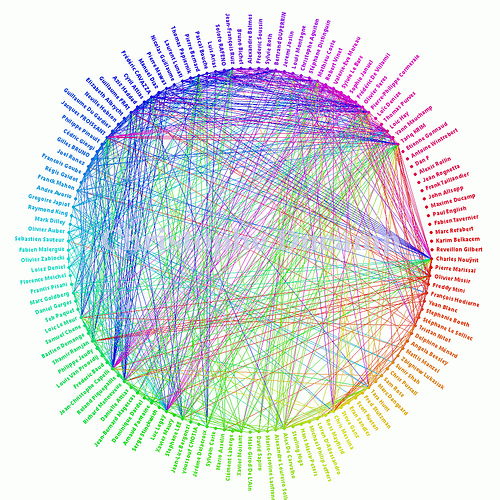
\includegraphics[scale=0.35]{facebookfriendwheel.jpg}
\end{slide}

\begin{slide}{Formalisation du problème}
Soit un graphe $G$ défini par un ensemble de sommets $V$ et un ensemble d'arêtes $E$. On cherche 

\vspace{0.5cm}

\pause

un sous-ensemble d'arêtes $F \subset E$:

\vspace{0.5cm}

\pause

tel que deux arêtes ne soient pas incidentes

\vspace{0.5cm}

\pause

de taille maximale

\end{slide}

\begin{slide}{{\`A} vous de jouer !}

A l'aide du fichier \texttt{data\_gen.py}, générez un graphe aléatoire à 20 sommets et 50 arêtes. Puis dessinez-le et cherchez graphiquement une allocation aussi grande que possible.

\end{slide}


\subsection{Rappel : Graphe et structures de données possibles}

\begin{slide}{3 Possibilités}

Un graphe peut être représenté par exemple comme :

\begin{itemize}

	\item une liste (voire un set) de sets de taille 2 (les arêtes)
	\item un dictionnaire de successeurs
	\item une classe spécifique (si vous connaissez la POO)

\end{itemize}

\end{slide}

\begin{slide}{Liste de sets}

\begin{center}
\begin{tikzpicture}
\draw (0,0) node[below left]{1} -- (0,1) node[above left]{2} -- (1,1) node[above right]{3} -- (1,0) node[below right]{4} -- (0,0) -- (1,1); 
\end{tikzpicture}
\end{center}

\texttt{g1 = [\{1,2\},\{1,3\},\{2,3\},\{3,4\},\{1,4\}]}

\end{slide}

\begin{slide}{Dictionnaire}

\begin{center}
\begin{tikzpicture}
\draw (0,0) node[below left]{1} -- (0,1) node[above left]{2} -- (1,1) node[above right]{3} -- (1,0) node[below right]{4} -- (0,0) -- (1,1); 
\end{tikzpicture}
\end{center}

\texttt{g1 = \{ 1:\{2,3,4\}, 2:\{1,3\}, 3:\{1,2,4\}, 4:\{1,3\} \}}

\end{slide}

\begin{slide}{Classe}

\Python{graph3}

\end{slide}

\begin{slide}{{\`A} vous de jouer !}

Sur l'exemple précédemment dessiné, concevez un algorithme glouton pour le problème du couplage maximum.

\end{slide}

\begin{slide}{Algorithme Glouton}

\Python{glouton}

\end{slide}

\begin{slide}{Chaîne augmentante}

\Python{testff}

\end{slide}

\subsection{Le problème du FLOT MAX}

\begin{slide}{Un réseau avec capacités}

\begin{center}
\begin{tikzpicture}[xscale=0.8,yscale=0.8]
	\coordinate(0) at (0,0);
	\coordinate(1) at (2,2);
	\coordinate(2) at (2,-2);
	\coordinate(3) at (4,2);
	\coordinate(4) at (4,-2);
	\coordinate(5) at (6,0);

	\draw[-latex] (0) node[left]{E} -- (1) node[above]{A} node[midway,left,gray] {7};
	\draw[-latex] (0) -- (3) node[above]{B} node[midway,right,gray] {2};
	\draw[-latex] (0) -- (4) node[below]{C} node[midway,left,gray] {5};
	\draw[-latex] (1) -- (2) node[below]{D} node[midway,right,gray] {3};
	\draw[-latex] (1) -- (3) node[midway,above left,gray] {1};
	\draw[-latex] (2) -- (5) node[right]{S} node[midway,right,gray] {3};
	\draw[-latex] (3) -- (5) node[midway,left,gray] {5};
\end{tikzpicture}
\end{center}

\end{slide}

\begin{slide}{Un flot sous-optimal}

\begin{center}
\begin{tikzpicture}[xscale=0.8,yscale=0.8]
	\coordinate(0) at (0,0);
	\coordinate(1) at (2,2);
	\coordinate(2) at (2,-2);
	\coordinate(3) at (4,2);
	\coordinate(4) at (4,-2);
	\coordinate(5) at (6,0);

	\draw[-latex,red] (0) node[left]{E} -- (1) node[above]{A} node[midway,left,gray] {7} node[midway,above,red] {1};
	\draw[-latex] (0) -- (3) node[above]{B} node[midway,right,gray] {2};
	\draw[-latex] (0) -- (4) node[below]{C} node[midway,left,gray] {5};
	\draw[-latex] (1) -- (2) node[below]{D} node[midway,right,gray] {3};
	\draw[-latex,red] (1) -- (3) node[midway,above left,gray] {1} node[midway,above right,red] {1};
	\draw[-latex] (2) -- (5) node[right]{S} node[midway,right,gray] {3} ;
	\draw[-latex,red,] (3) -- (5) node[midway,left,gray] {5} node[midway,right,red] {1};
\end{tikzpicture}
\end{center}

\end{slide}

\begin{slide}{Un flot optimal}

\begin{center}
\begin{tikzpicture}[xscale=0.8,yscale=0.8]
	\coordinate(0) at (0,0);
	\coordinate(1) at (2,2);
	\coordinate(2) at (2,-2);
	\coordinate(3) at (4,2);
	\coordinate(4) at (4,-2);
	\coordinate(5) at (6,0);

	\draw[-latex,red] (0) node[left]{E} -- (1) node[above]{A} node[midway,left,gray] {7} node[midway,above,red] {4};
	\draw[-latex,red] (0) -- (3) node[above]{B} node[midway,right,gray] {2} node[pos=0.7,right,red] {2};
	\draw[-latex] (0) -- (4) node[below]{C} node[midway,left,gray] {5};
	\draw[-latex,red] (1) -- (2) node[below]{D} node[midway,right,gray] {3} node[midway,left,red] {3};
	\draw[-latex,red] (1) -- (3) node[midway,above left,gray] {1} node[midway,above right,red] {1};
	\draw[-latex,red] (2) -- (5) node[right]{S} node[midway,right,gray] {3} node[midway,above,red] {3} ;
	\draw[-latex,red,] (3) -- (5) node[midway,left,gray] {5} node[midway,right,red] {3};
\end{tikzpicture}
\end{center}

\end{slide}


\begin{slide}{{\`A} vous de jouer !}

\begin{center}
\begin{tikzpicture}

\node (1) at (0,0){Ainur};
\node (2) at (0,1){Béatrice};
\node (3) at (0,2){Claude};
\node (4) at (0,3){Denis};
\node (5) at (4,0){Eléonore};
\node (6) at (4,1){François};
\node (7) at (4,2){Genki};
\node (8) at (4,3){Hussein};
\draw (1) -- (5);
\draw (1) -- (7);
\draw (2) -- (5);
\draw (2) -- (6);
\draw (2) -- (8);
\draw (3) -- (6);
\draw (4) -- (6);
\draw (4) -- (8);

\end{tikzpicture}
\end{center}

Comment ramener un problème de MATCHING dans un graphe biparti comme celui-ci à un problème de FLOT MAX ?

\end{slide}

\begin{slide}{Solution}

\begin{center}
\begin{tikzpicture}

\node (0) at (-2,1.5){E};
\node (9) at (6,1.5){S};
\node (1) at (0,0){Ainur};
\node (2) at (0,1){Béatrice};
\node (3) at (0,2){Claude};
\node (4) at (0,3){Denis};
\node (5) at (4,0){Eléonore};
\node (6) at (4,1){François};
\node (7) at (4,2){Genki};
\node (8) at (4,3){Hussein};
\draw (1) -- (5);
\draw (1) -- (7);
\draw (2) -- (5);
\draw (2) -- (6);
\draw (2) -- (8);
\draw (3) -- (6);
\draw (4) -- (6);
\draw (4) -- (8);
\draw (0) -- (1);
\draw (0) -- (2);
\draw (0) -- (3);
\draw (0) -- (4);
\draw (9) -- (5);
\draw (9) -- (6);
\draw (9) -- (7);
\draw (9) -- (8);

\end{tikzpicture}
\end{center}

Toutes les arêtes ont une capacité 1.

\end{slide}

\subsection{Ford-Fulkerson / Edmonds}

\begin{slide}{Chaîne augmentante}

\begin{tikzpicture}

\node (1) at (0,0){Ainur};
\node (2) at (0,1){Béatrice};
\node (3) at (0,2){Claude};
\node (4) at (0,3){Denis};
\node (5) at (4,0){Eléonore};
\node (6) at (4,1){François};
\node (7) at (4,2){Genki};
\node (8) at (4,3){Hussein};
\draw[ultra thick,red] (1) -- (5);
\draw (1) -- (7);
\draw (2) -- (5);
\draw[ultra thick,red] (2) -- (6);
\draw (2) -- (8);
\draw (3) -- (6);
\draw (4) -- (6);
\draw[ultra thick,red] (4) -- (8);

\end{tikzpicture}

\end{slide}

\begin{slide}{Deux sommets isolés}

\begin{tikzpicture}

\node (1) at (0,0){Ainur};
\node (2) at (0,1){Béatrice};
\node[shape=rectangle,fill=blue!40] (3) at (0,2){Claude};
\node (4) at (0,3){Denis};
\node (5) at (4,0){Eléonore};
\node (6) at (4,1){François};
\node[shape=rectangle,fill=blue!40] (7) at (4,2){Genki};
\node (8) at (4,3){Hussein};
\draw[ultra thick,red] (1) -- (5);
\draw (1) -- (7);
\draw (2) -- (5);
\draw[ultra thick,red] (2) -- (6);
\draw (2) -- (8);
\draw (3) -- (6);
\draw (4) -- (6);
\draw[ultra thick,red] (4) -- (8);

\end{tikzpicture}

\end{slide}

\begin{slide}{Une chaîne alternée}

\begin{tikzpicture}

\node (1) at (0,0){Ainur};
\node (2) at (0,1){Béatrice};
\node[shape=rectangle,fill=blue!40] (3) at (0,2){Claude};
\node (4) at (0,3){Denis};
\node (5) at (4,0){Eléonore};
\node (6) at (4,1){François};
\node[shape=rectangle,fill=blue!40] (7) at (4,2){Genki};
\node (8) at (4,3){Hussein};
\draw[ultra thick,red] (1) -- (5);
\draw[ultra thick,blue] (1) -- (7);
\draw[ultra thick,blue] (2) -- (5);
\draw[ultra thick,red] (2) -- (6);
\draw (2) -- (8);
\draw[ultra thick,blue] (3) -- (6);
\draw (4) -- (6);
\draw[ultra thick,red] (4) -- (8);

\end{tikzpicture}

\end{slide}

\begin{slide}{Le cas non-biparti}

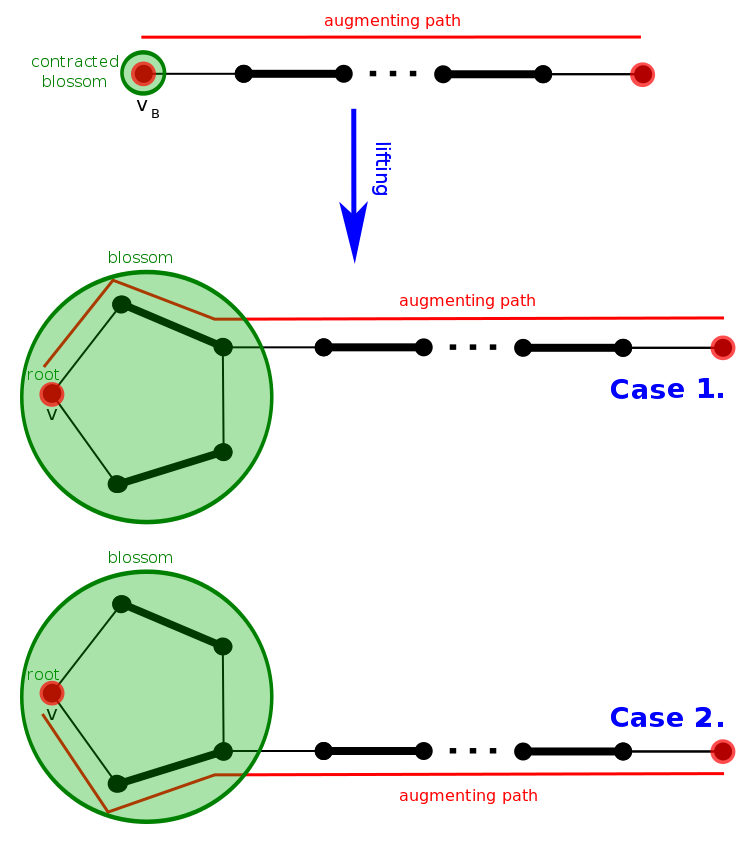
\includegraphics[scale=0.2]{Edmonds}

\end{slide}


\begin{slide}{{\`A} vous de jouer !}

1) Reprenez l'exemple graphique que vous avez construit précédemment et générez rapidement une solution quelconque (non optimale). Puis cherchez une sous-chaîne améliorante.

\vspace{0.3cm}

2) Récupérez le code complet de Ford-Fulkerson/Edmonds (par ex. sur wikipedia) et testez le sur un exemple simple.

\end{slide}


\subsection{Retour complexité + I/O en Python}


\begin{slide}{Complexité}

Les algorithmes de Ford-Fulkerson et Edmonds ont une complexité polynomiale (resp. $n\times m$ et $n^2\times m$).

\vspace{0.3cm}

Ilpeuvent donc tourner sur des instances incomparablement plus grandes qu'un algorithme exponentiel.

\end{slide}

\begin{slide}{Complexité}

On va pouvoir travailler sur des graphes contenant des milliers de sommets...\\

\vspace{0.3cm}

Naturellement, plus question de rentrer ces données manuellement.

\end{slide}

\begin{slide}{Lire un fichier}

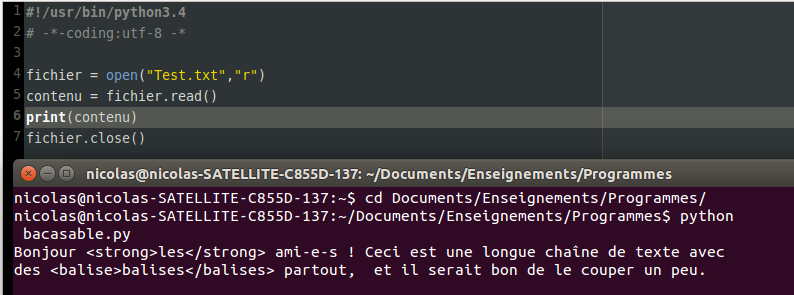
\includegraphics[scale=0.4]{./pyopenfile}

\end{slide}

\begin{slide}{{\'E}crire dans un fichier}

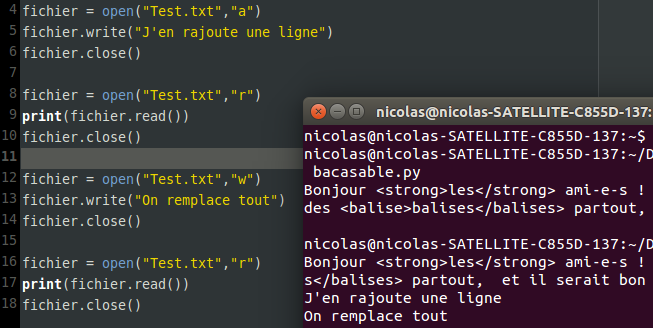
\includegraphics[scale=0.4]{./pywritefile}

\end{slide}

\part{Déterminer des préférences}

\section{Déterminer des préférences}

\subsection{Présentation de l'analyse multivariée}


\begin{slide}{Données monovariées}

\begin{tikzpicture}

\draw[-latex,thick] (-1,-1) -- (7,-1)node[below] {revenus};

\node[shape=rectangle,fill=red] (1) at (0,0){};
\node[shape=rectangle,fill=red] (2) at (1.8,0){};
\node[shape=rectangle,fill=red] (4) at (3,0){};
\node[shape=rectangle,fill=red] (4) at (3.4,0){};
\node[shape=rectangle,fill=red] (5) at (4.8,0){};
\node[shape=rectangle,fill=red] (6) at (6,0){};
\pause
\draw (1.6,0.3) rectangle (3.6,-0.3);
\draw (4.6,0.3) rectangle (6.2,-0.3);

\end{tikzpicture}

\end{slide}


\begin{slide}{Données bivariées}

\begin{tikzpicture}

\draw[-latex,thick] (-1,-1) -- (7,-1)node[below] {revenus};
\draw[-latex,thick] (-1,-1) -- (-1,4.5)node[left] {études};

\node[shape=rectangle,fill=red] (1) at (0,4){};
\node[shape=rectangle,fill=red] (2) at (1.8,1){};
\node[shape=rectangle,fill=red] (4) at (3,0.5){};
\node[shape=rectangle,fill=red] (4) at (3.4,3){};
\node[shape=rectangle,fill=red] (5) at (4.8,3.2){};
\node[shape=rectangle,fill=red] (6) at (6,1){};
\pause
\draw (1.6,1.3) rectangle (3.2,0.2);
\draw (3.2,2.7) rectangle (5,3.4);

\end{tikzpicture}

\end{slide}


\begin{slide}{Données multivariées}

Comment représenter sur un écran un classement selon des dizaines ou des milliers de critères ? 

\vspace{0.5cm}

Comment déterminer des compatibilités entre des individus représentés par autant de variables ?

\end{slide}

\begin{slide}{Réduction dimensionnelle}
\begin{center}
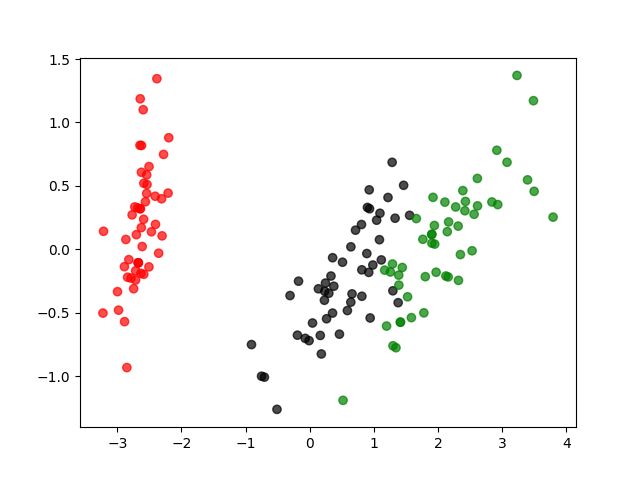
\includegraphics[scale=0.4]{iris_acp}
\end{center}
\end{slide}

\begin{slide}{Réduction dimensionnelle}
\begin{center}
\Python{acp}
\end{center}
\end{slide}


\begin{slide}{{\`A} vous de jouer !}

Importez le fichier \texttt{data2.csv} et essayez de construire une représentation ou de modéliser un graphe de compatibilité.

\end{slide}

\subsection{Construction de distances, principe et exemples}

\begin{slide}{Données numériques}

Normalisation (exemple) : 

$$x' = \frac{x-xmin}{xmax-xmin}$$

Agrégation (exemple) :

$$ d(X,Y) = \sqrt{\sum(x_i-y_i)^2} $$

\end{slide}

\begin{slide}{Données par modalités}

Distance binaire :

$$ d(X,Y) = \sharp \{ x_i \neq y_i \} = \sum_{x_i \neq y_i} 1 $$

Distance pondérée :

$$ d(X,Y) = \sum_{x_i \neq y_i} \omega_i $$

\end{slide}

\begin{slide}{Exemple}

$X$ : BLOND, BAC+5, MODEM, 43 ans

$Y$ : BLOND, BAC+2, NPA, 36 ans\\

\vspace{0.2cm}

\pause

$X'$ : BLOND, 0.6, MODEM, 0.7

$Y'$ : BLOND, 0.3, NPA, 0.55

\pause

$$d(X,Y) = \sqrt{0 + (0.6-0.3)^2 + 1 + (0.7-0.55)^2}$$

\end{slide}


\begin{slide}{{\`A} vous de jouer !}

Construisez une matrice de distances sur les données du fichier \texttt{data2.csv}.

\end{slide}

\subsection{Construction de graphes avec seuil simple}

\begin{slide}{Principe}

On fixe un seuil, par exemple $S=N/4$, où $N$ est le nombre de variables.

\pause

On considère que deux sommets doivent être reliés si et seulement si leur distance est inférieure au seuil.

$(X,Y) \in G \Longleftrightarrow d(X,Y) < S$

\end{slide}

\begin{slide}{Exemple}

$X$ : BLOND, 0.6, MODEM, 0.7\\
$Y$ : BLOND, 0.3, NPA, 0.55\\
$Z$ : BRUN, 0.5, LR, 0.8\\
$T$ : BRUN, 0.2, NPA, 0.2\\

\end{slide}

\begin{slide}{Exemple}

\begin{tabular}{|c|c|c|c|c|}
\hline
& X & Y & Z & T \\ \hline
X &\cellcolor{black!20} \color{black!20} 0.0&1.45&2.30&2.90 \\ \hline
Y &&\cellcolor{black!20} \color{black!20} 0.0&2.45&1.45 \\ \hline
Z &&&\cellcolor{black!20} \color{black!20} 0.0&1.90 \\ \hline
T &&&&\cellcolor{black!20} \color{black!20} 0.0 \\ \hline
\end{tabular}

\end{slide}

\begin{slide}{Exemple}

\begin{tabular}{|c|c|c|c|c|}
\hline
& X & Y & Z & T \\ \hline
X &\cellcolor{black!20} \color{black!20} 0.0&\cellcolor{red!50}{1.45}&2.3&2.9 \\ \hline
Y &&\cellcolor{black!20} \color{black!20} 0.0&2.45&\cellcolor{red!50}1.45 \\ \hline
Z &&&\cellcolor{black!20} \color{black!20} 0.0&\cellcolor{red!50}1.9 \\ \hline
T &&&&\cellcolor{black!20} \color{black!20} 0.0 \\ \hline
\end{tabular}

\end{slide}


\begin{slide}{{\`A} vous de jouer !}

1) Fixez un seuil et utilisez la matrice de l'exercice précédent pour construire des proximités entre les individus. \\

\vspace{0.3cm}

2) Essayez de produire le graphe correspondant.

\end{slide}

\subsection{MATCHING vs CLUSTERING (cliques)}

\begin{slide}{Rappel : le MATCHING}
Soit un graphe $G$ défini par un ensemble de sommets $V$ et un ensemble d'arêtes $E$. On cherche 

\vspace{0.5cm}

\pause

un sous-ensemble d'arêtes $F \subset E$:

\vspace{0.5cm}

\pause

tel que deux arêtes ne soient pas incidentes

\vspace{0.5cm}

\pause

de taille maximale

\end{slide}


\begin{slide}{Rappel : le CLUSTERING}
Soit un graphe $G$ défini par un ensemble de sommets $V$ et un ensemble d'arêtes $E$. On cherche 

\vspace{0.5cm}

\pause

Une division de $V$ en sous-ensembles disjoints $V_1$, $V_2$, $V_3$...

\vspace{0.5cm}

\pause

avec un maximum d'arêtes à l'intérieur de chaque $V_i$

\vspace{0.5cm}

\pause

et un minimum à l'extérieur, entre les différents $V_i$.

\end{slide}

\begin{slide}{Exemple}

\begin{tikzpicture}

\node[shape=rectangle,fill=red] (1) at (0,0){};
\node[shape=rectangle,fill=red] (2) at (0,1){};
\node[shape=rectangle,fill=red] (3) at (1,2){};
\node[shape=rectangle,fill=red] (4) at (2,1){};
\node[shape=rectangle,fill=red] (5) at (4,2){};
\node[shape=rectangle,fill=red] (6) at (5,3){};
\node[shape=rectangle,fill=red] (7) at (6,2.5){};
\node[shape=rectangle,fill=red] (8) at (7,1){};
\node[shape=rectangle,fill=red] (9) at (5.5,1.5){};
\draw (1) -- (2);
\draw (1) -- (3);
\draw (2) -- (3);
\draw (3) -- (4);
\draw (3) -- (5);
\draw (4) -- (1);
\draw (5) -- (6);
\draw (5) -- (7);
\draw (7) -- (8);
\draw (6) -- (9);
\draw (5) -- (9);
\pause
\draw[dashed] (-0.3,-0.3) rectangle (2.3,2.3);
\draw[dashed,color=red] (3.7,3.3) rectangle (5.8,1.2);
\draw[dashed] (5.7,2.8) rectangle (7.3,0.7); 

\end{tikzpicture}

\end{slide}

\begin{slide}{Différents types d'objectifs}

\begin{itemize}
\item Ne regrouper que des éléments tous deux à deux compatibles : 

$$x \in V_i, y \in V_i \Longrightarrow (x,y) \in G $$

\pause

\item Ratio inter/intra minimal :

$$ \min \frac{\sharp\{(x,y) \in G, x \in V_i, y \in V_j\}}{\sharp\{(x,y) \in G, x,y \in V_i\}}$$

\end{itemize}

\end{slide}


\begin{slide}{{\`A} vous de jouer !}

Trouvez un clustering pertinent sur l'exemple des exercices précédents.

\end{slide}


\subsection{La classification hiérarchique ascendante}

\begin{slide}{Principe}

On va procéder de façon itérative.

\pause

A chaque étape on regroupe les deux éléments les plus proches.

\pause

Le groupement ainsi constitué est considéré comme un pseudo-élément positionné en son barycentre.

\end{slide}


\begin{slide}{Exemple}

\begin{tikzpicture}

\node[shape=rectangle,fill=red] (1) at (0,0){};
\node[shape=rectangle,fill=red] (2) at (0,1){};
\node[shape=rectangle,fill=red] (3) at (1,2){};
\node[shape=rectangle,fill=red] (4) at (2,1){};
\node[shape=rectangle,fill=red] (5) at (4,2){};
\node[shape=rectangle,fill=red] (6) at (5,3){};
\node[shape=rectangle,fill=red] (7) at (6,2.5){};
\node[shape=rectangle,fill=red] (8) at (7,1){};
\node[shape=rectangle,fill=red] (9) at (5.5,1.5){};
\pause
\draw[dashed] (-0.3,-0.3) rectangle (0.3,1.3);
\pause
\draw[dashed] (4.7,2.2) rectangle (6.3,3.3);

\end{tikzpicture}

\end{slide}

\begin{slide}{Exemple}

\begin{tikzpicture}

\node[shape=rectangle,fill=red] (1) at (0,0){};
\node[shape=rectangle,fill=red] (2) at (0,1){};
\node[shape=rectangle,fill=red] (3) at (1,2){};
\node[shape=rectangle,fill=red] (4) at (2,1){};
\node[shape=rectangle,fill=red] (5) at (4,2){};
\node[shape=rectangle,fill=red] (6) at (5,3){};
\node[shape=rectangle,fill=red] (7) at (6,2.5){};
\node[shape=rectangle,fill=red] (8) at (7,1){};
\node[shape=rectangle,fill=red] (9) at (5.5,1.5){};
\draw[dashed] (-0.3,-0.3) rectangle (0.3,1.3);
\draw[dashed] (4.7,1.2) rectangle (6.3,3.3);
\pause
\draw[dashed] (0.7,0.7) rectangle (2.3,2.3);

\end{tikzpicture}

\end{slide}

\begin{slide}{Exemple}

\begin{tikzpicture}

\node[shape=rectangle,fill=red] (1) at (0,0){};
\node[shape=rectangle,fill=red] (2) at (0,1){};
\node[shape=rectangle,fill=red] (3) at (1,2){};
\node[shape=rectangle,fill=red] (4) at (2,1){};
\node[shape=rectangle,fill=red] (5) at (4,2){};
\node[shape=rectangle,fill=red] (6) at (5,3){};
\node[shape=rectangle,fill=red] (7) at (6,2.5){};
\node[shape=rectangle,fill=red] (8) at (7,1){};
\node[shape=rectangle,fill=red] (9) at (5.5,1.5){};
\draw[dashed] (-0.3,-0.3) rectangle (0.3,1.3);
\draw[dashed] (3.7,1.2) rectangle (6.3,3.3);
\draw[dashed] (0.7,0.7) rectangle (2.3,2.3);

\end{tikzpicture}

\end{slide}

\begin{slide}{{\`A} vous de jouer !}

Programmez un algorithme de classification hiérarchique ascendante. Testez-le sur l'exemple précédent (à partir de la table de distances).

\end{slide}

\subsection{Cartes auto-organisatrices}


\begin{slide}{}
	Qu'est-ce que c'est ?\\ \vspace{0.2cm}
	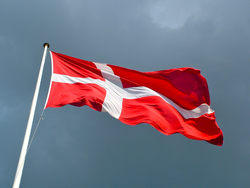
\includegraphics[scale=1]{danish_flag.png}
\end{slide}

\begin{slide}{}
	Quelle est son origine ?\\ \vspace{0.2cm}
	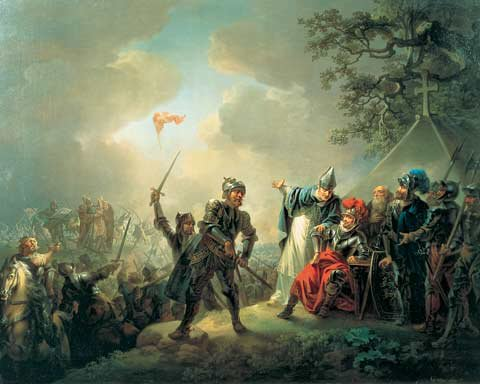
\includegraphics[scale=2.5]{Anders_Sunesen.jpg}
\end{slide}

\begin{slide}{La Livonie, XII\up{e}-XIII\up{e} siècles}
\begin{center}
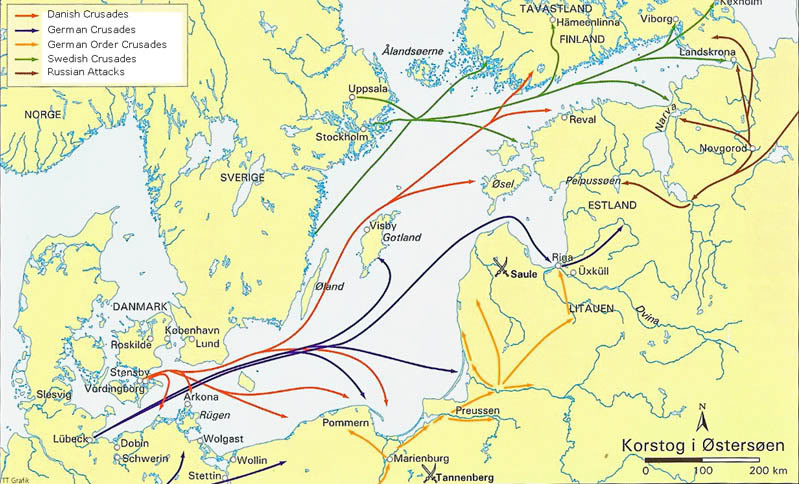
\includegraphics[scale=0.37]{crusades.jpg}
\end{center}
\end{slide}

\begin{slide}{Le texte d'Henri}
\begin{center}
\begin{tabular}{cc}
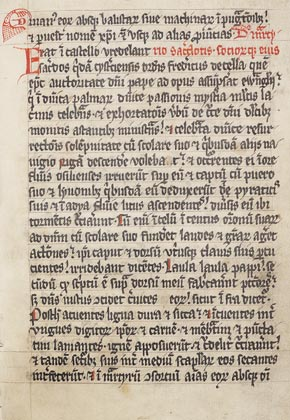
\includegraphics[scale=0.4]{HL.jpg} &
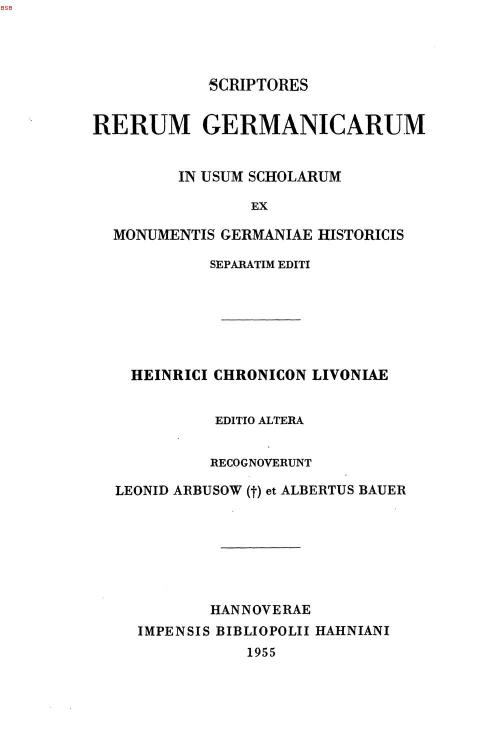
\includegraphics[scale=0.3]{MGH.jpeg}
\end{tabular}
\end{center}
\end{slide}

\begin{slide}{Saisie}

\begin{tabular}{lllll}
	D{\"u}nam{\"u}nde & Daugavgr{\=\i}va & N 57\up{o} 3' & E 24\up{o} 2' & 1186 \\
	D{\"u}nam{\"u}nde & Daugavgr{\=\i}va & N 57\up{o} 3' & E 24\up{o} 2' & 1186 \\
	D{\"u}nam{\"u}nde & Daugavgr{\=\i}va & N 57\up{o} 3' & E 24\up{o} 2' & 1191 \\
	Dorpat & Tartu & N 58\up{o} 23' & E 26\up{o} 43'& 1214 \\
	Dorpat & Tartu & N 58\up{o} 23' & E 26\up{o} 43'& 1217 \\
\end{tabular}

\end{slide}


\begin{slide}{la Livonie d'Henri}
\begin{center}
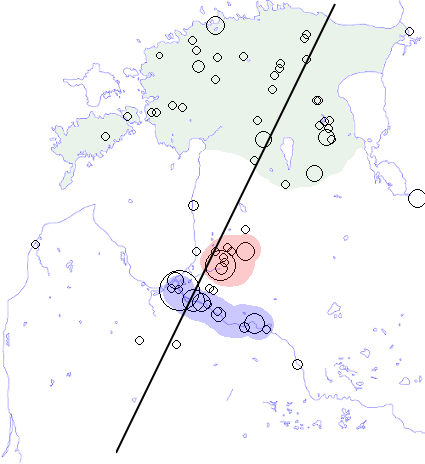
\includegraphics[scale=0.4]{HL_places_coloured_ACPpastel.png}
\end{center}
\end{slide}


\begin{slide}{Sous forme de graphe}
\begin{center}
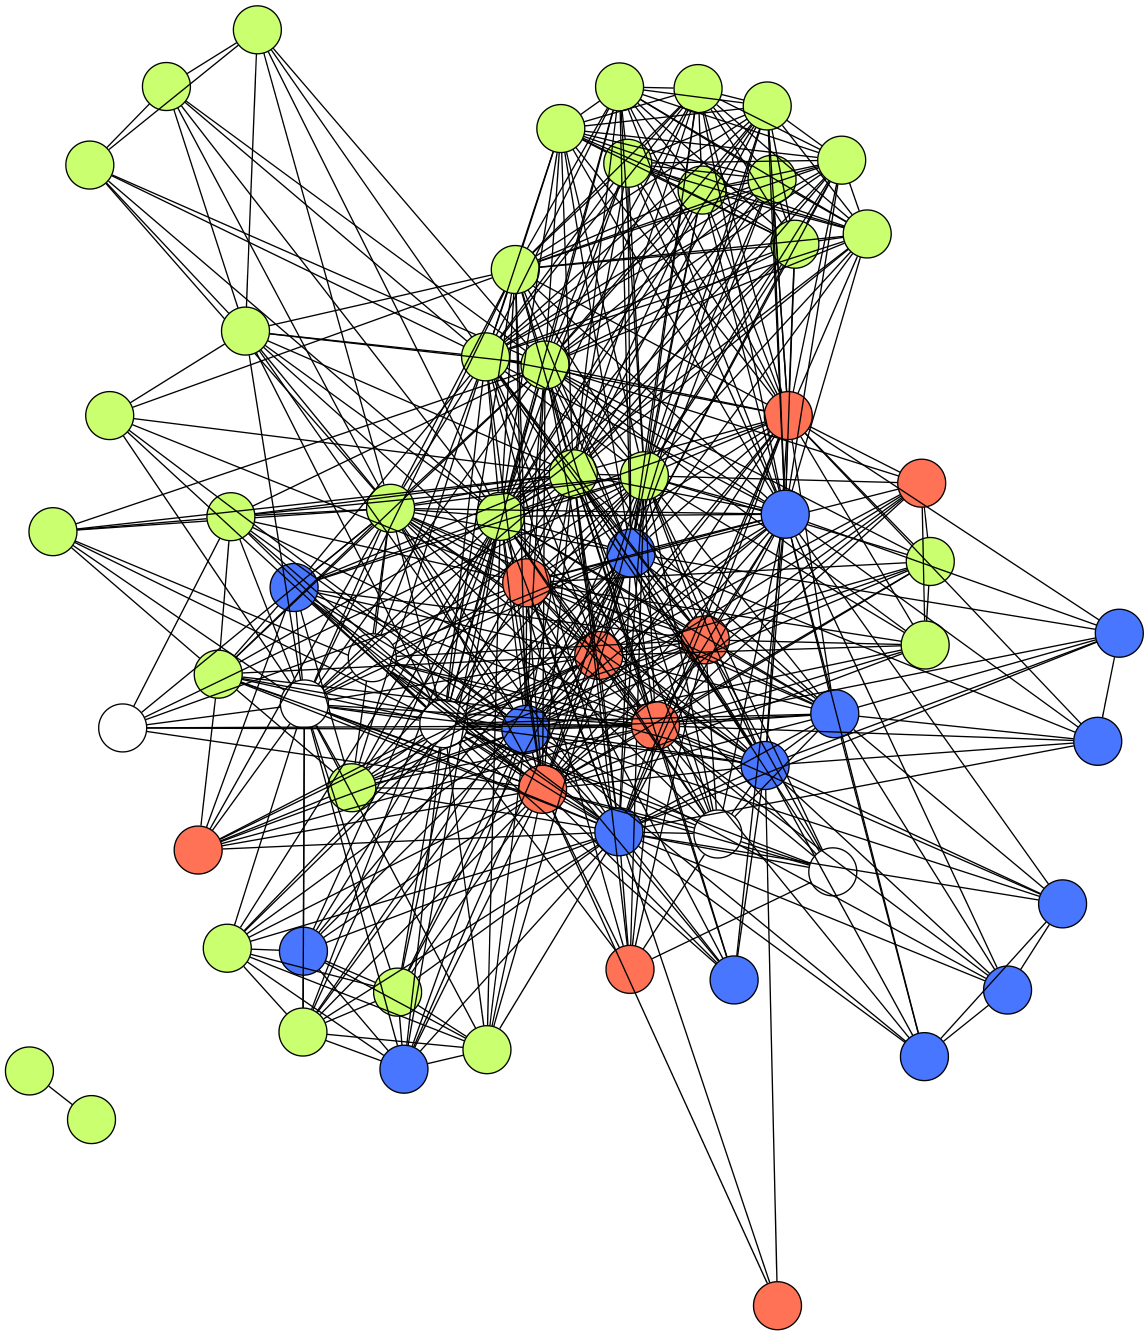
\includegraphics[scale=0.15,angle=270]{HL_places_graph.png}
\end{center}
\end{slide}

\begin{slide}{Carte de Kohonen}
\begin{center}
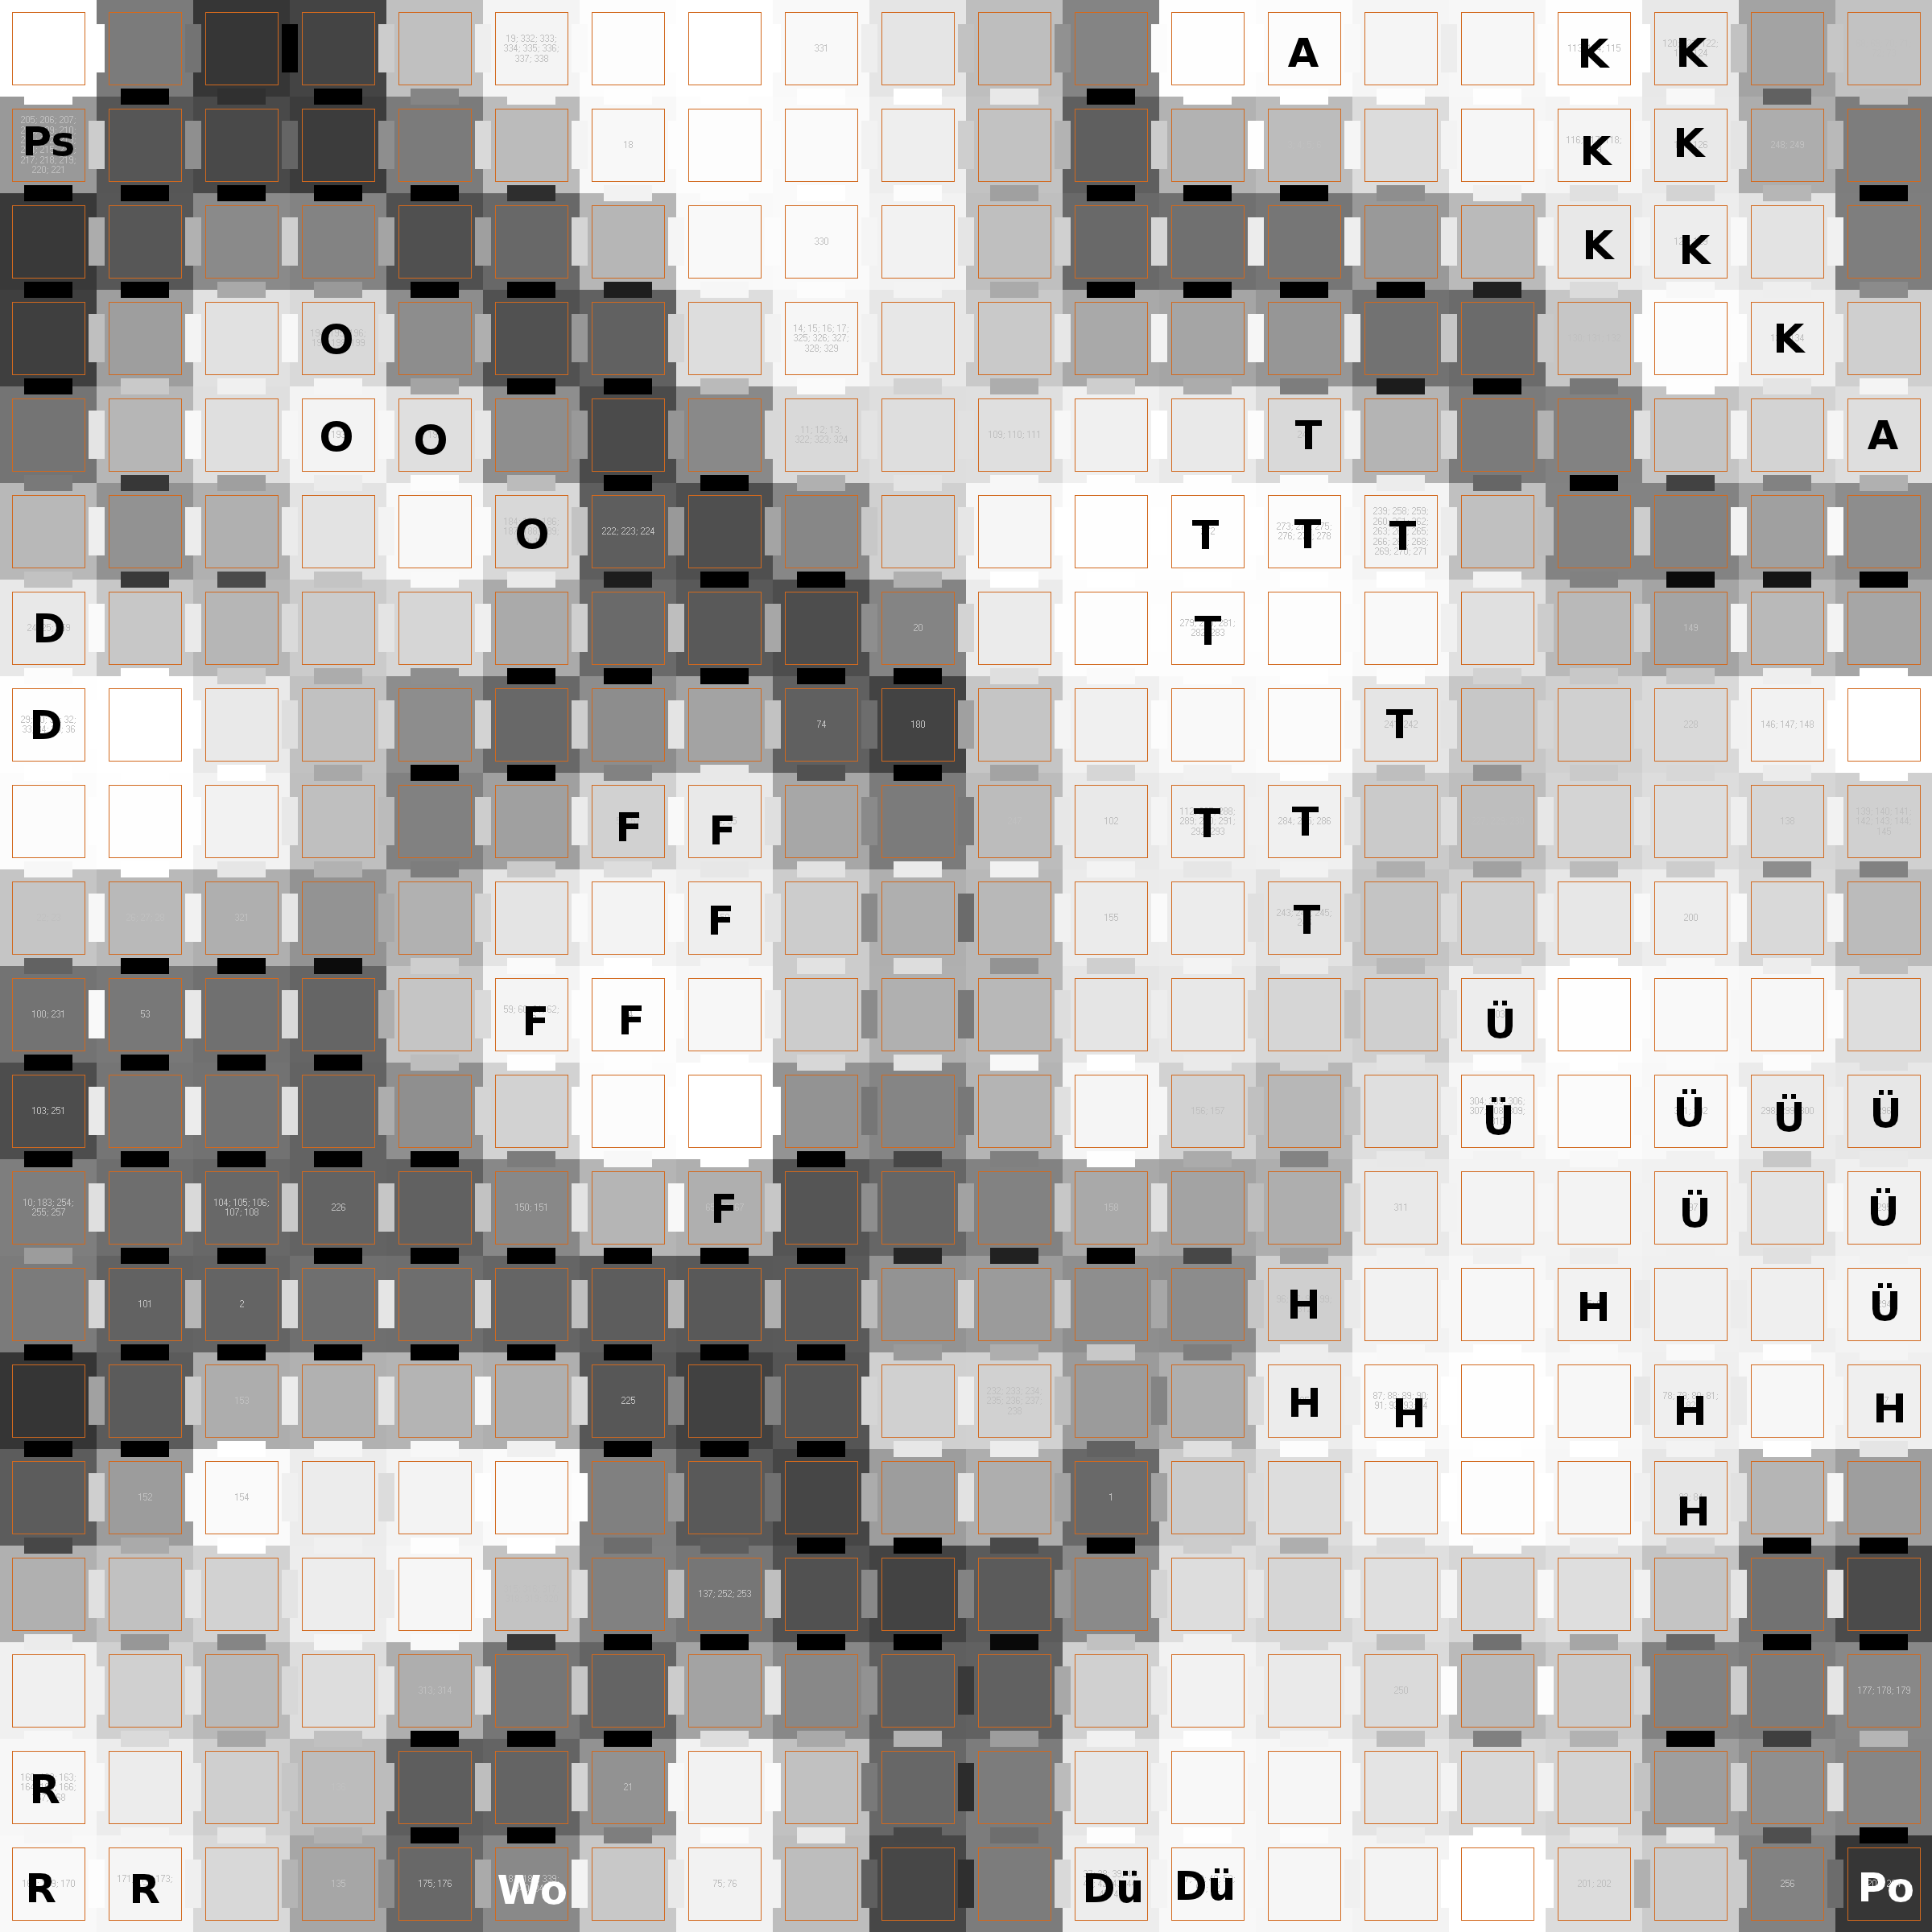
\includegraphics[scale=0.07]{HL_Kohonen.png}
\end{center}
\end{slide}


\begin{slide}{Distance à la rivière}
\begin{tabular}{cc}
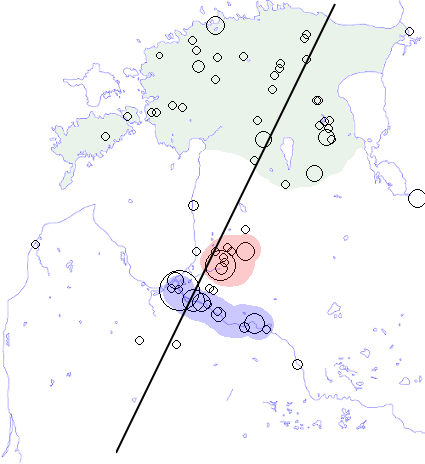
\includegraphics[scale=0.3]{HL_places_coloured_ACPpastel.png}&
\begin{tikzpicture}
\node[above right] (img4) at (0,0) {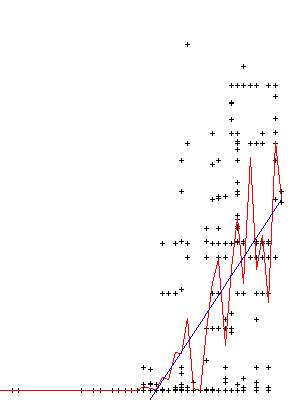
\includegraphics[scale=0.4]{Average_distance_to_river_with_reg.png}};
\draw[-latex] (6mm,10mm) -- +(8mm,0) node [below] {\footnotesize t(année)};
\draw[-latex] (6mm,10mm) -- +(0mm,8mm) node [above] {\footnotesize distance};
\node [right] at (0,0.4mm) {\tiny 1185};
\node [right] at (17.5mm,0.4mm) {\tiny 1205};
\node [right] at (35mm,0.4mm) {\tiny 1225};
\end{tikzpicture}
\end{tabular}
\end{slide}



\subsection{Optimisation : temps vs qualité du résultat}

\begin{slide}{Notions contradictoires}

Pour un problème donné, il faut souvent équilibrer plusieurs notions.

\begin{center}
\begin{tikzpicture}
\node[below] at (-3,0) {rapidité} ;
\node[below] at (0,-2){optimisation} ;
\draw[latex-latex] (-3,0) -- (3,0) node[below]{qualité};
\draw[latex-latex] (0,-2) -- (0,2) node[above]{généralité};
\end{tikzpicture}
\end{center}
\end{slide}

\begin{slide}{Arbitrages}

\begin{itemize}
\item Les solutions exhaustives fonctionnent toujours, mais leur coût est prohibitif.
\pause
\item Les algorithmes polynomiaux exacts comme FF n'existent que sur un nombre limité de problèmes.
\pause
\item Dans les autres cas (clustering par exemple), on se rabat sur des heuristiques et on essaie d'équilibrer rapidité et qualité.
\pause
\item Et évaluer cette dernière est souvent en soi un problème difficile...

\end{itemize}

\end{slide}

\begin{slide}{{\`A} vous de jouer !}

Quelle est la complexité respective des algorithmes vus tout au long de ce cours ?

\end{slide}

\end{document}